\section{\_\-yaml\_\-::tokens::ValueToken Class Reference}
\label{class__yaml___1_1tokens_1_1ValueToken}\index{_yaml_::tokens::ValueToken@{\_\-yaml\_\-::tokens::ValueToken}}
Inheritance diagram for \_\-yaml\_\-::tokens::ValueToken:\nopagebreak
\begin{figure}[H]
\begin{center}
\leavevmode
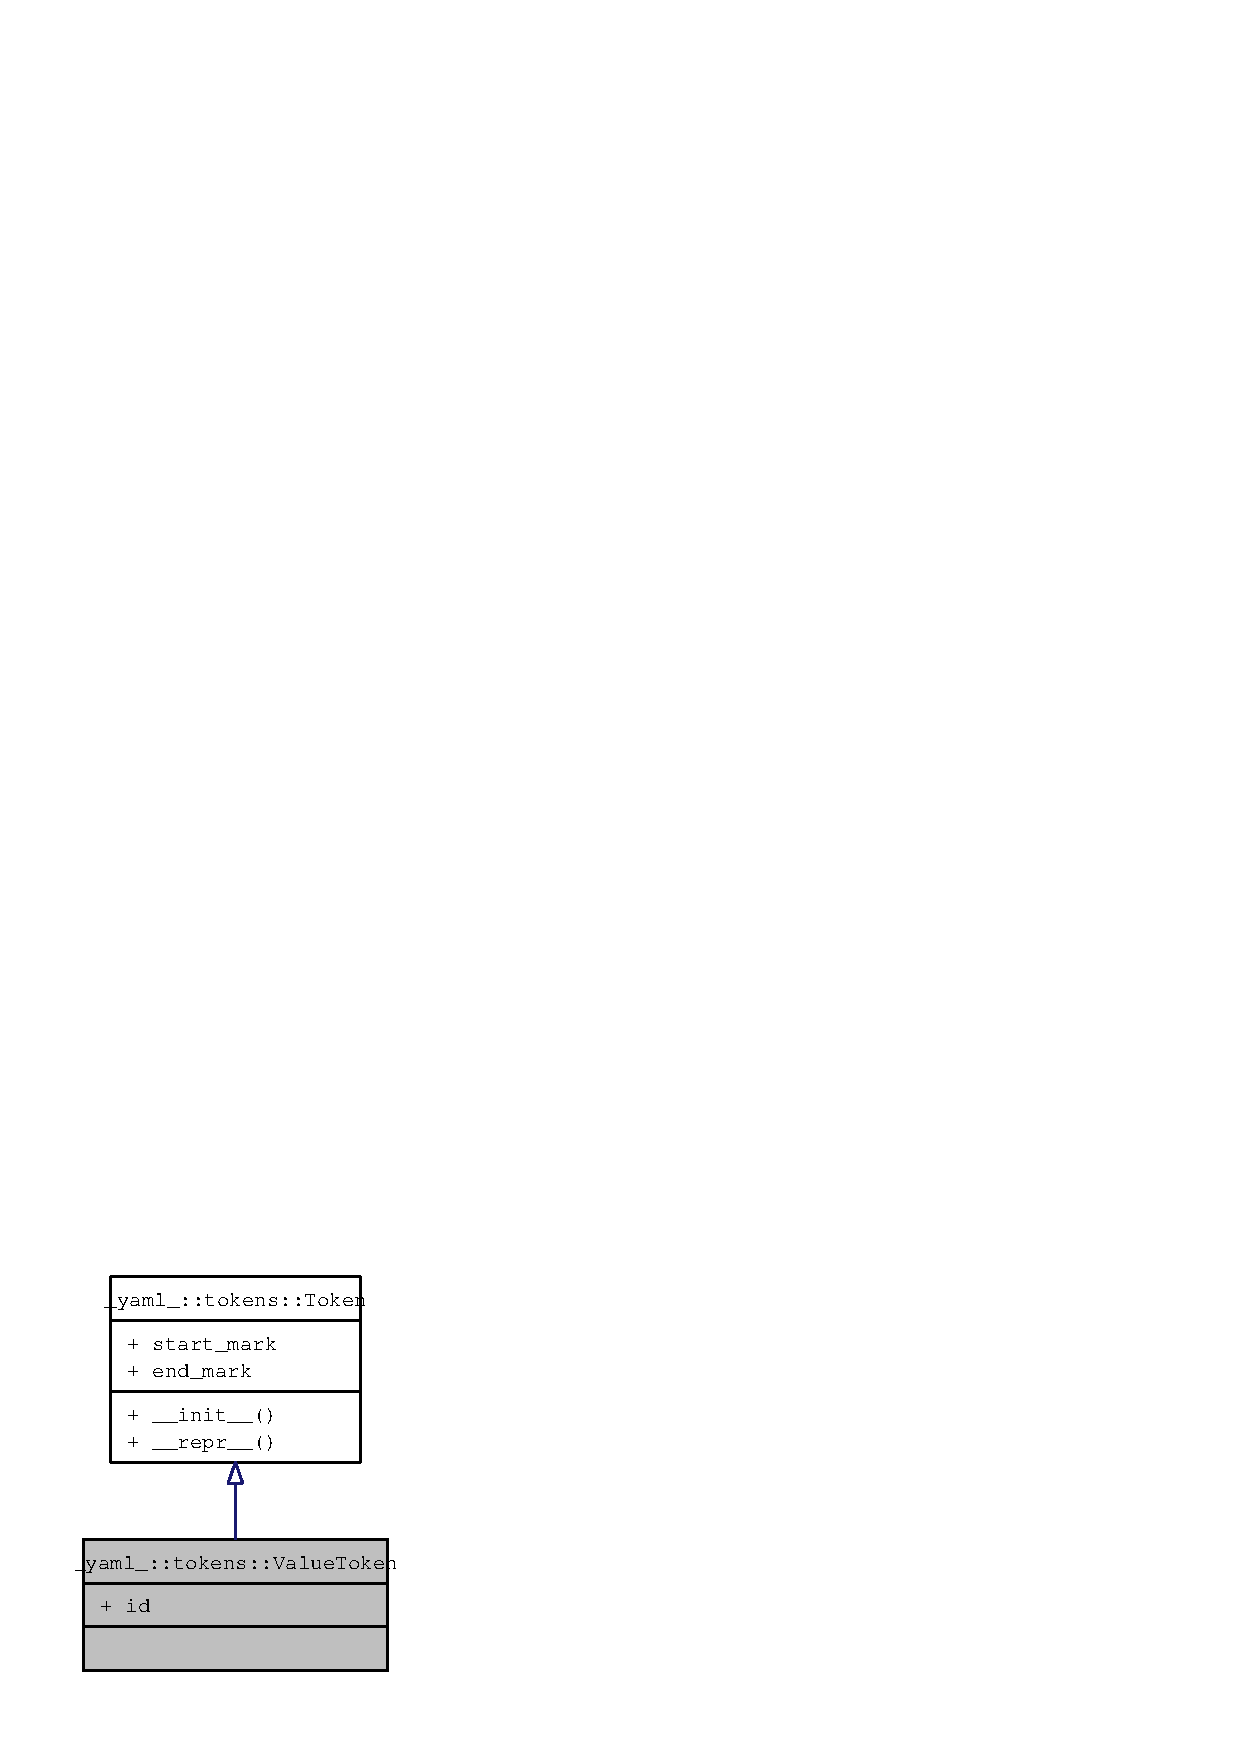
\includegraphics[width=95pt]{class__yaml___1_1tokens_1_1ValueToken__inherit__graph}
\end{center}
\end{figure}
Collaboration diagram for \_\-yaml\_\-::tokens::ValueToken:\nopagebreak
\begin{figure}[H]
\begin{center}
\leavevmode
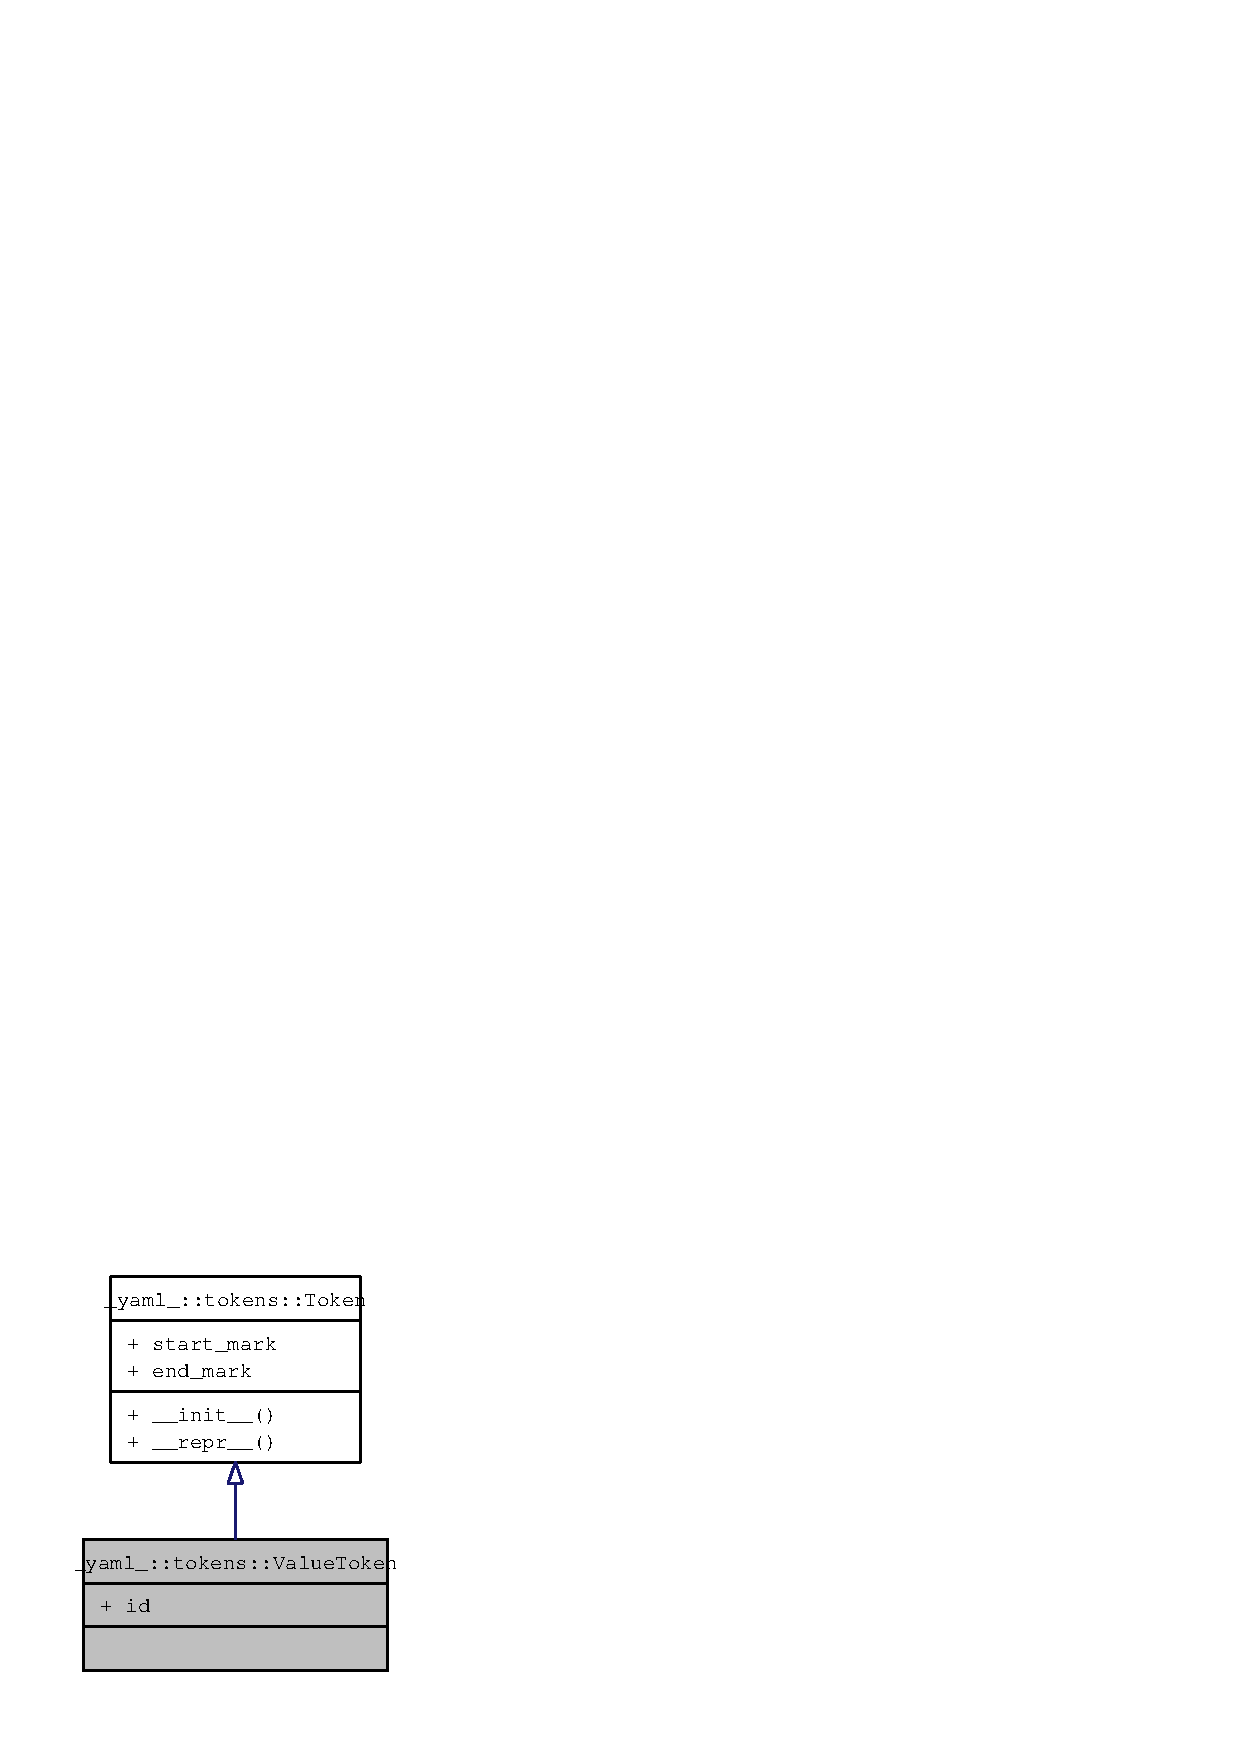
\includegraphics[width=95pt]{class__yaml___1_1tokens_1_1ValueToken__coll__graph}
\end{center}
\end{figure}
\subsection*{Static Public Attributes}
\begin{CompactItemize}
\item 
string {\bf id} = ':'
\end{CompactItemize}


\subsection{Detailed Description}


Definition at line 66 of file tokens.py.

\subsection{Member Data Documentation}
\index{_yaml_::tokens::ValueToken@{\_\-yaml\_\-::tokens::ValueToken}!id@{id}}
\index{id@{id}!_yaml_::tokens::ValueToken@{\_\-yaml\_\-::tokens::ValueToken}}
\subsubsection{\setlength{\rightskip}{0pt plus 5cm}string {\bf \_\-yaml\_\-::tokens::ValueToken::id} = ':'\hspace{0.3cm}{\tt  [static]}}\label{class__yaml___1_1tokens_1_1ValueToken_124c9a377ca712a566ba2155373cdde9}




Definition at line 67 of file tokens.py.

The documentation for this class was generated from the following file:\begin{CompactItemize}
\item 
/home/juan/xul\_\-ga/igap/\_\-yaml\_\-/{\bf tokens.py}\end{CompactItemize}
